\chapter{软件相关技术概述}

本章将对农业果实称重云端软件所使用的相关技术进行概述,包括 Spring 技术栈、YOLO 目标检测算法、基于 GTID 的主从复制技术、MQTT 消息传输协议以及 EMQX 网关框架这五种技术。

\section{Spring 技术栈}\label{sec:spring}

农业果实称重云端软件使用 Spring 技术栈来构建整个后台服务,技术栈包括了核心的 Spring 框架,以及两个重要的基于 Spring 的框架:Spring Security 和 Spring Boot。

\begin{figure}[H]
    \centering
    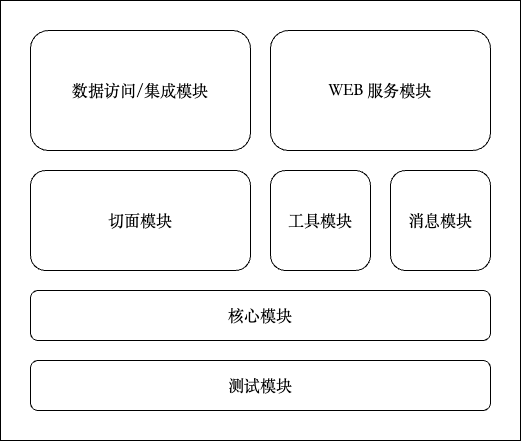
\includegraphics[width=\linewidth]{../design/out/Spring.png}
    \caption{Spring 七大模块}
    \label{fig:Spring}
\end{figure}

Spring 框架主要提供了七大模块的功能,分别是数据访问/集成模块、WEB服务模块、切面模块、工具模块、消息模块、核心模块以及测试模块,如图\ref{fig:Spring}所示;Spring Security 框架为软件提供了可靠的安全保障,确保了外部请求的安全性;Spring Boot 框架提供了简化应用开发和配置的能力,帮助快速构建和部署云端应用。

Spring 框架中的核心模块提供了 IOC(控制反转)和 DI (依赖注入)这两大功能;切面模块提供了 AOP (面向切面编程)支持;数据访问/集成模块主要提供了对象关系映射、事务、数据库连接、Java 消息服务以及对象 XML 映射这五个功能;Web 服务模块为应用提供了编解码、过滤器、跨域、WebFlux(响应式 Web 编程)、WebMVC(模型-视图-控制器模式)等功能;工具模块则为应用提供了服务监控、日志记录等扩展功能;消息模块提供了丰富易用的消息队列集成;测试模块则为应用提供了强大的单元测试支持\cite{Spring-框架概述}。

\begin{figure}
    \centering
    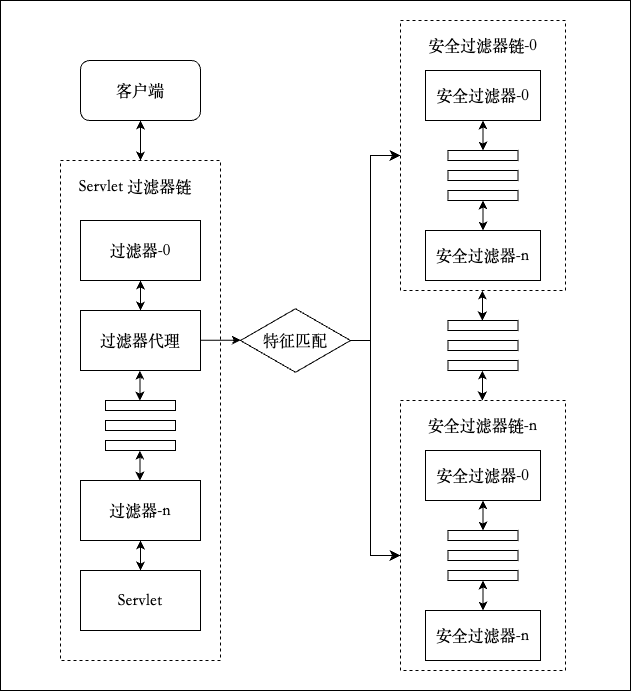
\includegraphics[width=0.8\linewidth]{../design/out/Spring-Security.png}
    \caption{Spring Security 请求过滤规则}
    \label{fig:Spring-Security}
\end{figure}

Spring Security 是 Spring 框架的安全扩展,专门用于解决应用的安全需求,通过与 Spring 的各个模块的集成,提供了一种高度灵活且易于配置的安全方案。Spring Security 提供了强大而灵活的安全过滤器,用于对用户进行认证和授权,其请求过滤规则如图\ref{fig:Spring-Security}所示,图中左侧的请求链是 Servlet 定义的过滤器链,右侧的请求链是 Spring Security 定义的安全过滤器链。客户端发起一个 HTTP 请求,请求首先到达 Servlet 过滤器链,其中过滤器0至过滤器n是普通的 Servlet 过滤器,通常用于执行非安全相关的任务如日志记录、性能监控、数据压缩等。Spring Security 所提供的过滤器代理委托者将会在 Servlet 过滤器链中拦截到该请求,将请求委托给过滤器代理,过滤器代理将根据请求的特征选择一个匹配的安全过滤器链,依次对请求进行处理(例如身份验证、授权等)。如果所有过滤器都允许该请求通过,则请求最终到达 Servlet 进行业务逻辑处理。Servlet 生成响应,响应同样会经过滤器链返回给客户端。如果在安全过滤器链的任何阶段,请求未能通过安全检查(例如身份验证失败或未授权),则会根据配置返回相应的错误响应\cite{Spring-Security-架构设计}。

Spring Boot 是建立在 Spring 框架之上的一款开源开发工具,旨在简化基于 Spring 的应用程序在构建、配置和部署过程中的复杂性。它通过提供自动化配置(Auto-Configuration)、开箱即用的起步依赖(Starter Dependencies)以及内嵌式服务器(如 Tomcat、Jetty 等),极大地降低了开发者在搭建 Spring 应用时的门槛\cite{Spring-Boot-概述}。

Spring Boot 采用“约定优于配置”的理念,提供了大量合理的默认设置,使开发者无需手动编写冗长的 XML 或注解配置,从而能够更加专注于业务逻辑的实现。此外,Spring Boot 还集成了丰富的监控与管理功能(如 Actuator 模块),可用于实时监控应用运行状态,提升系统的可维护性与稳定性。

在农业果实称重云端软件中,引入 Spring Boot 不仅提高了开发效率,还优化了系统的部署流程和可扩展性,使得后台服务能够快速构建并稳定运行于云端环境中。

综上所述,农业果实称重云端软件采用的 Spring 技术栈通过 Spring、Spring Security 和 Spring Boot 的紧密结合,提供了强大的功能支持和灵活的扩展性。

\section{YOLO 目标检测算法}\label{sec:yolo}

YOLO(You Only Look Once)是一种高效的目标检测算法,因其速度快、精度高的特点,在计算机视觉领域被广泛应用于实时目标检测任务\cite{Lin2019}。在农业果实称重云端软件中,应用 YOLO 来训练果实图像检测模型,实现果实种类的检测与识别。YOLO 的检测原理可以从图像划分、目标预测、损失函数和后处理四个方面阐述。

(1)图像划分:YOLO 将输入的图像划分为多个网格单元,各单元分别预测中心点落在单元内的目标。这种划分方式使得算法能够快速定位目标的大致位置,提高检测效率\cite{Liu2023-yolov8}。

(2)目标预测:对于每个网格单元,YOLO 预测多个边界框和对应的类别概率。边界框包含了目标的位置信息,通常用四个坐标值表示。类别概率表示该边界框内目标属于各个类别的可能性\cite{Liu2023-yolov8}。

(3)损失函数:YOLO 采用一种多任务损失函数,综合优化模型参数,涵盖边界框回归、类别分类和物体置信度等多个目标检测任务\cite{Liu2023-yolov8}。损失函数通常由分类损失和回归损失组成。分类损失用于衡量模型对目标类别的预测准确性,回归损失用于衡量模型对目标边界框的预测准确性。

(4)后处理:在预测完成后,YOLO 通常采用一些后处理方法,如非极大值抑制(Non-Maximum Suppression,NMS)或软非极大值抑制(Soft-NMS, Soft Non-Maximum Suppression)\cite{Lin2019},来去除重复的检测结果,提高检测的准确性。

\section{基于 GTID 的主从复制技术}\label{sec:gtid}

在农业果实称重云端软件中,使用了 MySQL 数据库来存储大量数据,数据存储分为主库存储和从库存储。主库完成数据的读写,而从库只进行数据的读取。为实现主从库数据的一致性,采用了基于全局事务标识符 (GTID, Global Transaction Identifier) 的主从复制技术来完成数据同步操作。GTID 由服务器全局唯一标识符(UUID, Universally Unique Identifier) 和事务编号组成,是一个在 MySQL 数据库中用于唯一标识一个事务的标识符。

\begin{figure}
    \centering
    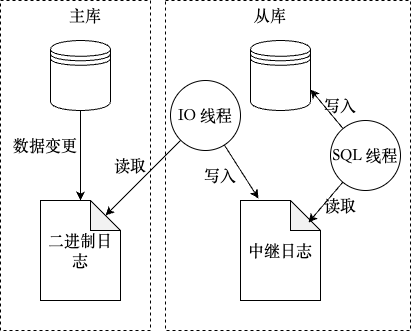
\includegraphics[width=\linewidth]{../design/out/GTID-Replication.png}
    \caption{主从复制流程}
    \label{fig:GTID-Replication}
\end{figure}

MySQL 所实现的主从复制技术性能优越,其内置的复制流量压缩选项可将总网络流量最多减少 20\%\cite{shehzad2020networkfootprintreplicationpopular}。其主从复制的流程如图\ref{fig:GTID-Replication}所示,左侧为主库,右侧为从库,具体执行解释如下:

1、主库在执行事务时,会为每个事务分配一个唯一的 GTID,并将该 GTID 记录在二进制日志中。

2、从库连接到主库后,读取主库二进制日志并将其写入本地的中继日志。根据其中的 GTID 来判断哪些事务已经执行过,哪些事务需要执行。如果一个事务的 GTID 不在从库的已执行事务集合中,从库就会执行该事务。

3、从库在执行事务时,也会为每个事务分配一个 GTID,并将其记录在自己的二进制日志中。这样,从库也可以作为其他从库的主库,实现级联复制\cite{MySQL-Liu2022}。

\section{MQTT 消息传输协议}\label{sec:mqtt}

MQTT(Message Queuing Telemetry Transport)即消息队列遥测传输协议,是一种轻量的消息传输协议。本软件采用 MQTT 作为称重消息的发布/订阅的通信协议,使用 EMQX(Erlang MQTT Broker) 作为 MQTT 消息发布服务器。EMQX 是开源软件,不仅性能表现优越,而且支持多种版本的 MQTT 协议\cite{dizdarevic2023engineeringexperimentallybenchmarkingopen}。在软件中,发送 MQTT 消息上传称重信息具有以下优势:

(1)低带宽和低功耗:MQTT 协议采用轻量消息格式与高效发布/订阅机制,适用于带宽受限、能耗敏感的物联网环境。对于电子秤等设备,可在网络资源有限或移动场景下稳定传输称重数据,降低通信负载与能耗\cite{Jia2015}。

(2)实时性和可靠性:MQTT 协议通过引入 QoS(Quality of Service,服务质量)机制,实现了对消息传输可靠性的灵活控制。根据不同应用场景的需求,MQTT 提供了三种 QoS 级别\cite{Jia2015},分别如下:

QoS 0(最多一次):消息最多发送一次,且不保证消息一定到达目标。适用于对实时性要求极高、但可容忍数据丢失的场景;

QoS 1(至少一次):保证消息至少成功传送一次,但可能会重复接收。适用于需要确保消息送达,但可以接受重复的业务场景;

QoS 2(仅一次):确保消息恰好传送一次,既不会丢失,也不会重复。适用于对消息传输可靠性和唯一性要求极高的关键场景。

由于农业果实称重云端软件在处理称重信息时要求消息必须被可靠接收且仅被消费一次,因此应选择 QoS 2 级别,以确保称重数据在网络传输过程中不会出现丢失或重复处理的情况,从而保证系统数据的一致性与准确性。

(3)易于扩展和集成:MQTT 协议可以轻松地与其他物联网协议进行集成,如 CoAP、WebSocket、HTTP 等。MQTT 协议的发布/订阅模式支持大规模的设备连接和数据传输,适用于构建物联网应用平台。例如,在智慧农业大棚测控系统中,采用 MQTT 协议将大棚内的测控系统和物联网云平台进行结合,通过移动终端访问云服务器数据库,实现了对农业大棚的实时监测和控制\cite{Liang2020}。

\section{EMQX 网关框架}\label{sec:emqx}

在农业果实称重云端软件中,为支持更多电子秤协议的接入,采用了 EMQX 网关框架,将多种不同物联网应用层协议在网关处转换为 MQTT 协议,使用 MQTT 协议继续进行后续的通信。框架提供了统一的用户层接口和会话/连接管理。各个协议的客户端有独立的认证器和监控器\cite{EMQX-Gateway}。其整体的架构如图\ref{fig:EMQX-Gateway}所示,左侧展现了 EMQX 网关的分层架构,右侧展现的是 MQTT 发布/订阅核心组成。在 EMQX 网关分层架构中,左下角显示了包括 MQTT-SN、Stomp、CoAP 等在内的多种协议,这些协议有着独立的认证器来完成认证和监控器来进行客户端级别的指标统计功能。

\begin{figure}
    \centering
    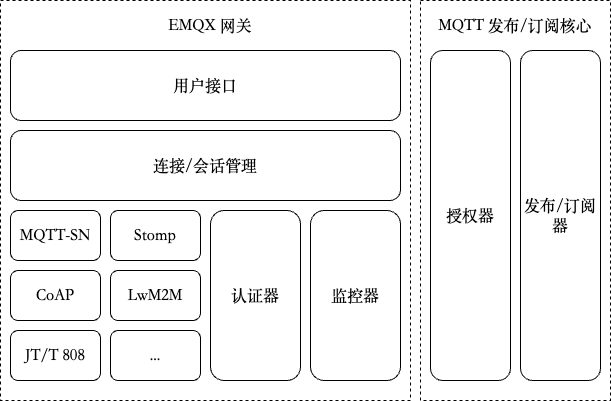
\includegraphics[width=\linewidth]{../design/out/EMQX-Gateway.png}
    \caption{EMQX 网关框架架构}
    \label{fig:EMQX-Gateway}
\end{figure}

不同协议的消息进入网关后,首先完成认证,认证通过后将会进行消息模型的转换,将消息内容转换成为 MQTT 格式的内容,并以 MQTT 协议进行后续的通信。通过 MQTT 授权器完成授权功能,最后执行发布和订阅动作。

\section{本章小结}

本章围绕农业果实称重云端软件所涉及的核心技术进行了系统性概述。首先,介绍了构建后台服务所采用的 Spring 技术栈,包括 Spring 框架的模块化设计、Spring Security 提供的安全机制以及 Spring Boot 对应用配置与部署流程的简化,这些技术共同构建起了稳定、灵活且易于扩展的软件基础架构。其次,分析了 YOLO 目标检测算法的核心原理与应用方式,展示了其在果实图像识别中的高效性与准确性,为图像数据的智能处理提供了技术支撑。

在数据同步方面,详细阐述了基于 GTID 的 MySQL 主从复制机制,确保了主从数据库间的数据一致性与高可靠性,为大规模数据的持续写入与读取提供了基础保障。随后,本章介绍了 MQTT 消息传输协议的优势,特别是在低带宽、高实时性需求的物联网环境中,借助其灵活的 QoS 机制,有效提升了称重信息的传输效率与稳定性。最后,通过对 EMQX 网关框架的分析,阐明了其在多协议接入、消息转换与认证授权方面的关键作用,为系统的多样化设备接入提供了强有力的技术支持。

综上所述,本章所介绍的五项关键技术从系统架构、智能识别、数据同步、通信传输及协议兼容等多个维度,为农业果实称重云端软件的稳定运行、高效处理和可持续拓展奠定了坚实的技术基础。